\chapter{Robot Firmware Implementation}
\label{Chapter 5}
\lhead{Chapter 5. \emph{Robot Firmware Implementation}}

With the creation of the software embedded Bluetooth stack and the \textit{ExplorerBot} test robot platform hardware, it was neccesary to integrate these two components into a functional prototype. By using the Bluetooth stack in a real-world, practical application while it was being developed, the quality, effectiveness and completeness of the stack could be evaluated.

\section{Build Dependencies}

To match the Bluetooth stack, each module was written in the C language, and targeted at the free open source AVR-GCC compiler and avr-libc library. A standard \textit{makefile} included with the firmware allows for command line control over the building of the project files into a set of binaries which can then be programmed into the target microcontroller for use via the command \texttt{make all}. The following tools are required to build the firmware under Windows:

\begin{itemize}
	\item The \textbf{WinAVR 20100101} release download, or Windows binaries of the \textbf{GNU Shell Utilities}
	\item The latest \textbf{AVR Toolchain} release from Atmel (Included with Atmel's free \textit{AVRStudio 5} software)
\end{itemize}

Under Debian Linux environments, the following packages are required:

\begin{itemize}
	\item \textbf{gcc-avr} 
	\item \textbf{binutils-avr}
	\item \textbf{avr-libc}
	\item \textbf{avrdude}
\end{itemize}

Which can be installed via the command prompt using the command \texttt{sudo apt-get install gcc-avr binutils-avr avr-libc avrdude}.

\section{Firmware Overview}

The completed firmware of the \textit{ExplorerBot} prototype was developed in a modular manner, to match the corresponding hardware components. This top-down methodology ensured that each portion of the firmware could be mocked up, tested and integrated as needed. Additionally, seperating out the firmware components into logical modules gave the final firmware a level of flexibility which should allow for easy modification to suit any hardware changes made to those of the prototype. The completed set of modules (see Figure \ref{fig:robotblockfw}) served as the complete firmware for the robot.

\begin{figure}[H]
	\vspace{1em}
	\centering
		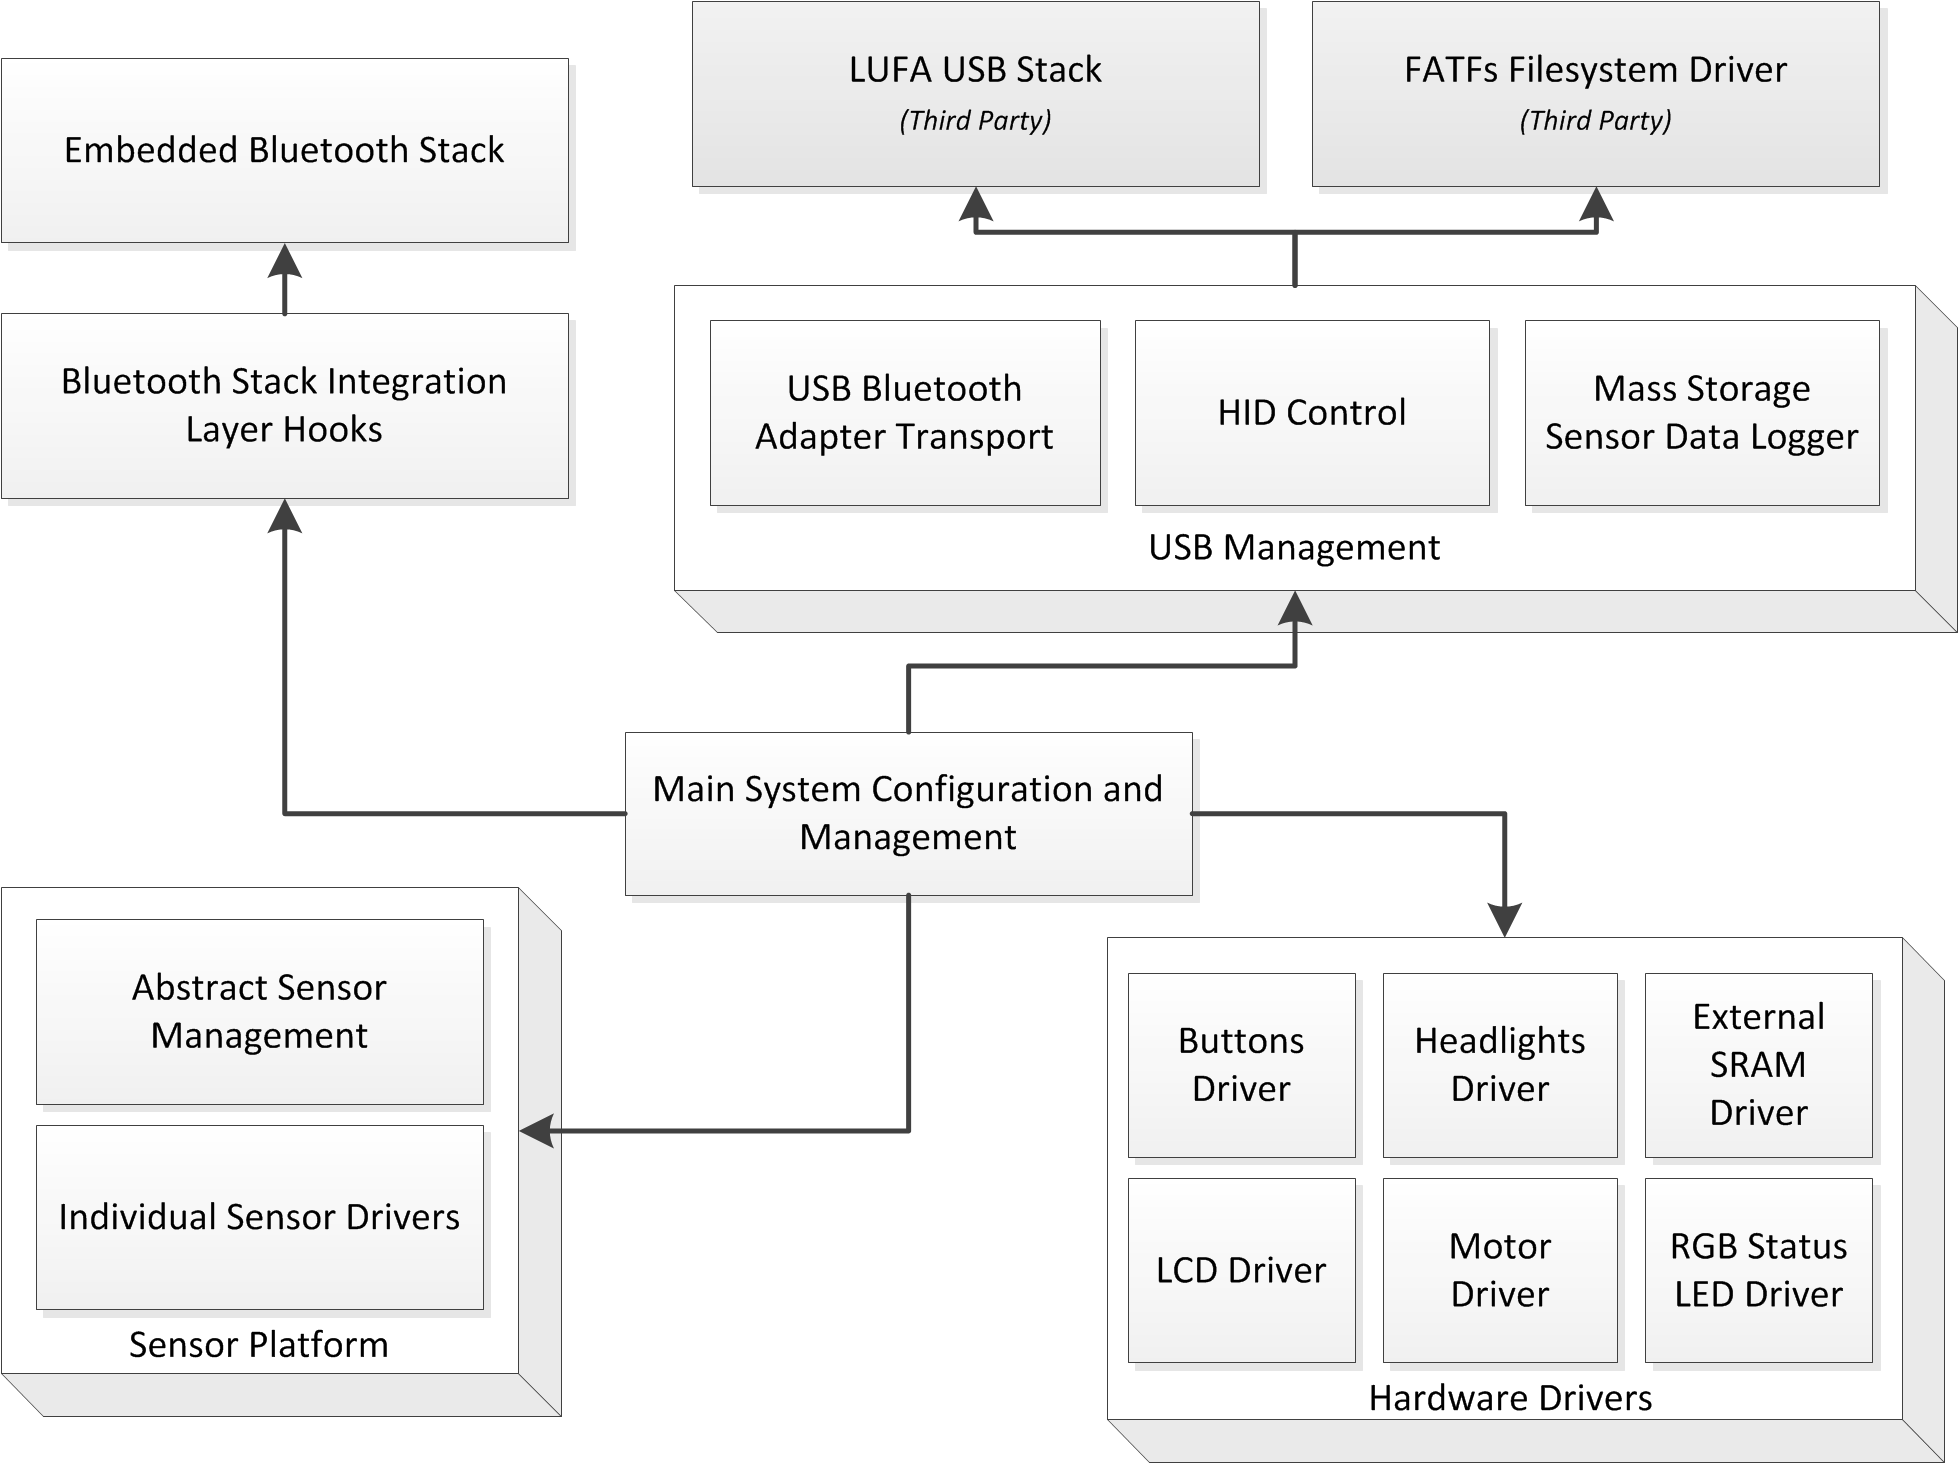
\includegraphics[width=140mm]{FirmwareBlockDiagram.png}
	\rule{35em}{0.5pt}
	\caption[Firmware Block Diagram]{Robot Firmware Block Diagram}
	\label{fig:robotblockfw}
\end{figure}

\section{Firmware Modules}

In this section, each of the robot firmware's main software modules are listed and described in additional detail so that the overall design and implementation of the firmware can be further understood.

\FloatBarrier
\subsection{Main System Control and Configuration}

% TODO

\FloatBarrier
\subsection{Hardware Drivers}

At the point at which the abstract software in the device needed to interact with the physical board hardware, a set of hardware abstraction drivers was created. These drivers served to encapsulate the functionality of the physical hardware and expose that functionality to the rest of the firmware via a set of basic control API functions. Not every driver sought to expose all the possibile abilities of the hardware; due to time constraints only those features actually required by the prototype robot firmware were implemented in most cases.

\FloatBarrier
\subsection{Sensor Platform}

As the robot contained an (optional) set of physical environment sensors, a "Sensor Platform" module was created to logically encapsulate all aspects of the sensors - from initialization and updates, to data formatting of the retrieved values - into a single package that could be integrated into the rest of the project easily, but also remain extendable enough that it could also be re-used in other future projects. Comprising the sensor platform is two layers; one, the abstract sensor management layer, and two, the physical sensor drivers.

\FloatBarrier
\subsubsection{Abstract Sensor Management}

While the robot's auxillery sensor boards (the Atmel \textit{Inertial One} and \textit{Pressure One}) contained several different sensor ICs with very different characteristics, the Sensor Platform module was designed to abstract these differences out from the rest of the firmware. This abstraction was achieved by providing a pair of simple initialization and update functions, and a consistent structure for the retrieved sensor data. An additional pair of functions were written to convert the retrieved sensor values into a Comma Seperated Values (CSV) format, the retrived data could be automatically streamed out to one or more logical consumers. Missing sensors (either not mounted or faulty) are automatically ignored by the sensor platform once the call to their initialization function has failed to complete.

Unfortunately, this abstraction led to one notable problem; as each sensor has a variety of configuration parameters which are specific to that particular device (or physical property it measures) an abstract interface for sensor configuration could not easily be written. While this could be solved with additional design and planning, for the purposes of the project a decision was made to instead fix each sensor's configuration to sane defaults inside the physical sensor drivers, and not provide a method to alter these parameters on the fly.

The C language structure used to encapsulate the state of a single sensor is shown in Listing \ref{lst:sensorentry}. This structure definition is instantiated as an array inside the sensor platform, with one entry then being dedicated to each physical property being measured (as distinct from each physical sensor IC). In the case of the ITG3200 Gyroscope, the internal temperature sensor was also used as well as the orientation data - in this particular case, the temperature sensor was assigned a second sensor structure entry in the sensor structure array.

\lstinputlisting[float=tbph,caption={Sensor Platform's Abstract Sensor entry structure definition.},label={lst:sensorentry}]{./Figures/SensorPlatformEntry.c}

Of note is the use of a C \textit{union} to contain the retrieved sensor data, as either a single \lstinline{int32_t} signed 32-bit integer value, or a triplicate of three \lstinline{int16_t} signed 16-bit integers. The use of this union minimises the amount of memory used by each sensor entry, as the two styles of returned data can overlap physically in RAM as they are mutually exclusive (see Figure \ref{fig:sensorentry}). For sensors returning only a single 32-bit value, the sensor initialization function sets the corresponding \lstinline{SingleAxis} item in the structure so that the platform knows how to extract and format the retrieved data.

\begin{figure}[tbph]
	\vspace{1em}
	\centering
		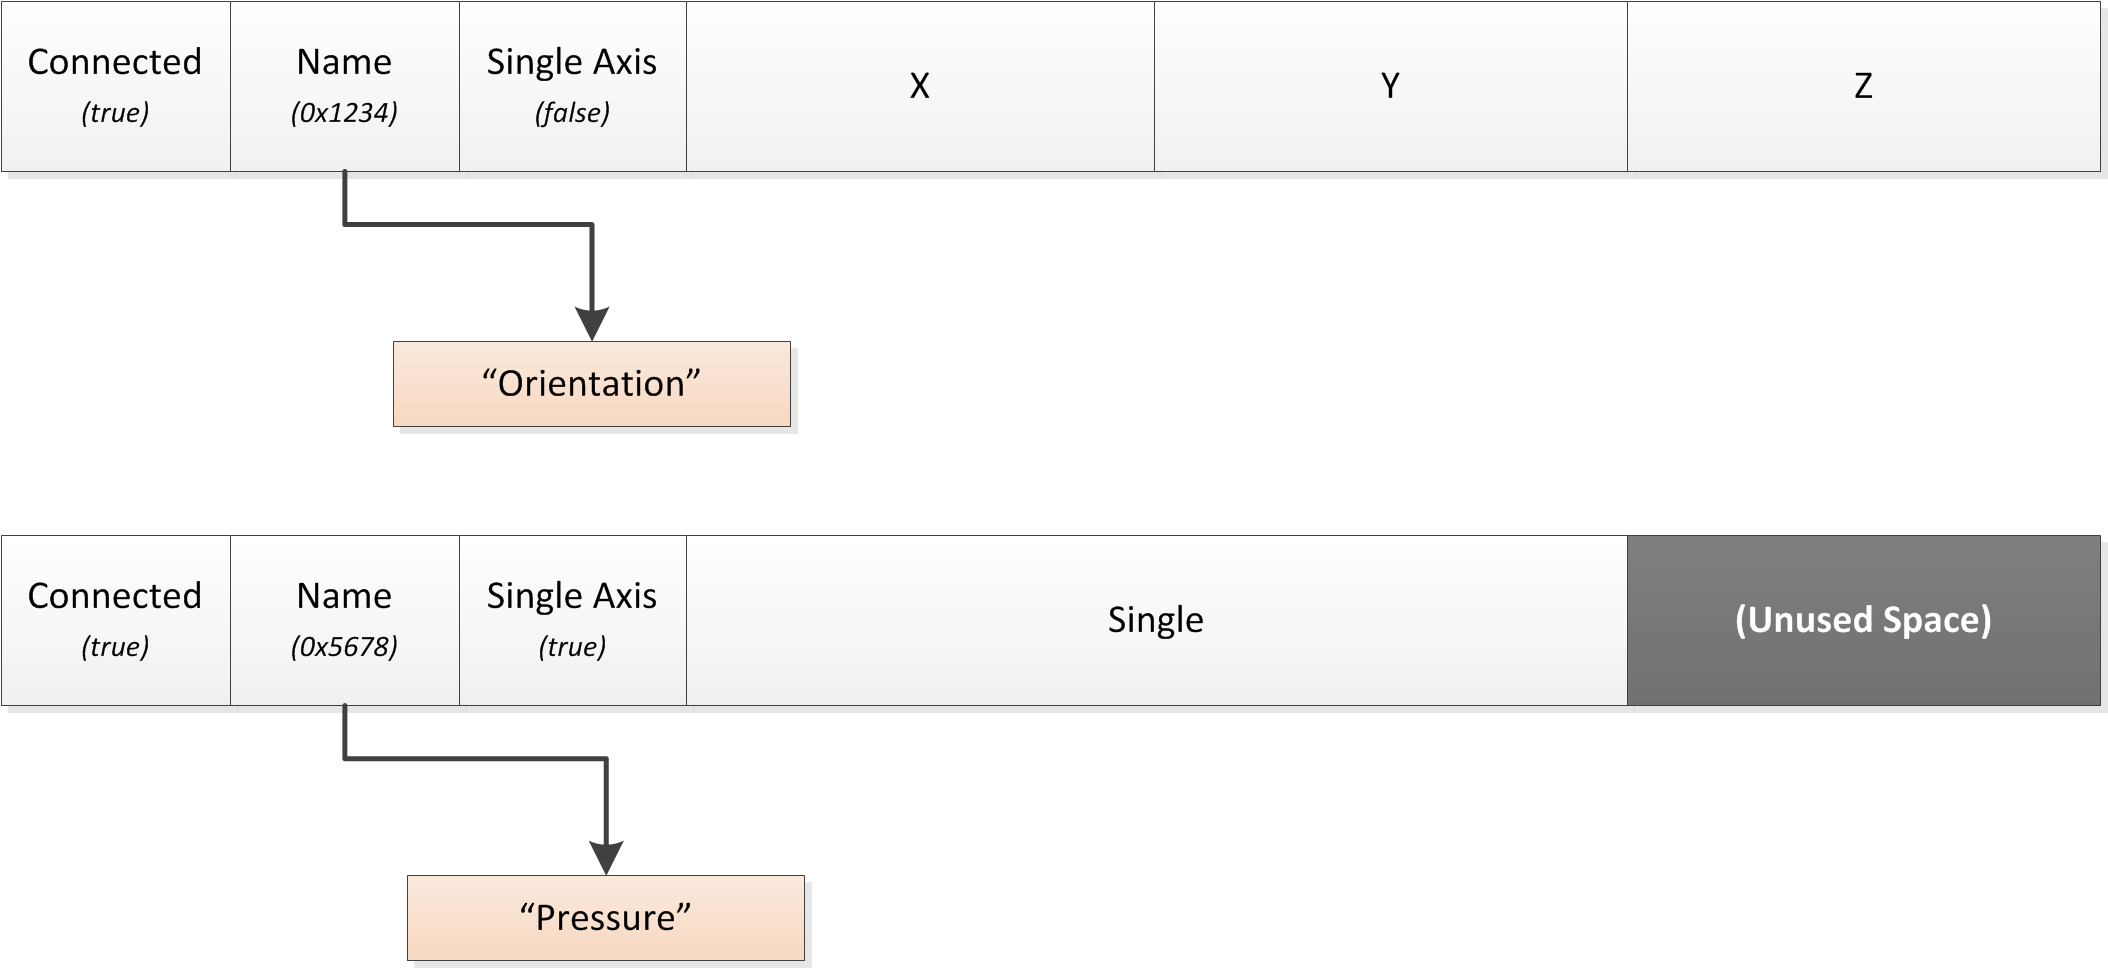
\includegraphics[width=130mm]{SensorPlatformEntry.png}
	\rule{35em}{0.5pt}
	\caption[Sensor Platform Entry Structure Diagram]{Diagram showing the layout of the Sensor Platform Entry structure in memory for triple axis (\textit{top}) and single axis (\textit{bottom}) sensors.}
	\label{fig:sensorentry}
\end{figure}

\FloatBarrier
\subsubsection{Individual Sensor Drivers}

Each individual sensor connected to the board requires an individual sensor driver, specific to that make and model of sensor IC.

\FloatBarrier
\subsection{USB Management}

% TODO

\FloatBarrier
\subsubsection{Bluetooth Adapters}

% TODO

\FloatBarrier
\subsubsection{HID Devices}

% TODO

\FloatBarrier
\subsubsection{Mass Storage Devices}

% TODO

\FloatBarrier
\subsection{Bluetooth Management}

% TODO

\FloatBarrier
\subsubsection{Stack Integration Layer}

% TODO

\FloatBarrier
\subsubsection{Bluetooth Stack}

% TODO

\FloatBarrier
\subsection{Third Party Modules}

% TODO

\FloatBarrier
\subsubsection{LUFA}

% TODO

\FloatBarrier
\subsubsection{FatFS}

% TODO
